\documentclass[../revisedMain.tex]{subfiles}
\begin{document}
	Estimating derivatives is not altogether too difficult. Remember that the derivative itself is just the limit of the difference quotient. If one needs to find the derivative, all one has to do is take the difference quotient at two known points to create a secant line. Because it is an estimate, one doesn't need to minimize $h$.$$\frac{f(x+h)-f(x)}{h}$$ It is also possible to ``eyeball'' a graph to estimate the derivative. For example:
	\begin{center}
		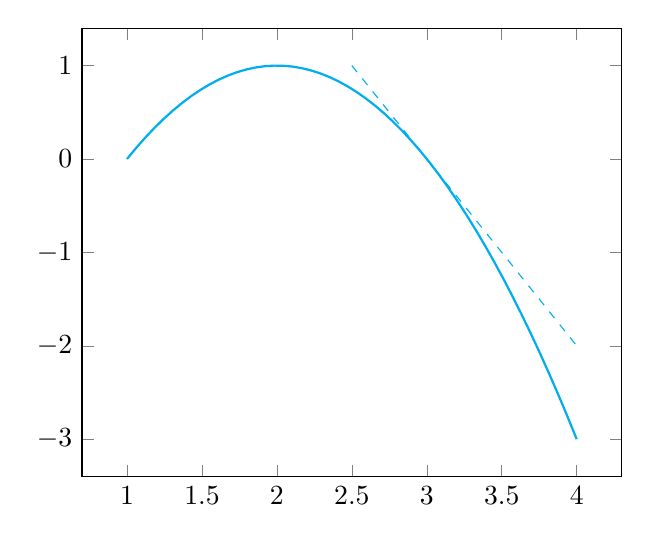
\begin{tikzpicture}
		\begin{axis}
		\addplot[domain=1:4,thick,cyan,samples=50]{-(x-2)^2+1};
		\addplot[domain=2.5:4,thin,cyan,dashed]{-2*x+6};
		\end{axis}
		\end{tikzpicture}
	\end{center}
	For the point (3,$f(3)$), the tangent line obviously has a negative slope. It is not too drastic so by a guesstimate, the slope must be greater than -3. The slope is also not too flat so it should be less than -1. Therefore, the derivative can be estimated to something around -2.
\end{document}
